\section{Mathematische Grundlagen}

\subsection{Vektorfelder}

\subsubsection{Divergenz}

$\boxed{\nabla\cdot\vec{F}=
\operatorname{div}\vec{F}=
\frac{\partial F}{\partial x}+
\frac{\partial F}{\partial y}+
\frac{\partial F}{\partial z}}$\\

Die Divergenz beschreibt die \textbf{Quellendichte} eines Skalarfeldes. \\
Interpretiert man ein Vektorfeld als Strömungsfeld,
so gibt die Divergenz für jede Stelle die Tendenz an, 
ob ein Teilchen in der Nähe zu diesem Punkt hin- bzw. von
diesem Punkt wegfliesst. \\
Es sagt damit aus, ob und wo das Vektorfeld Quellen (Divergenz grösser als Null) oder
Senken (Divergenz kleiner als Null) hat. \\
Ist die Divergenz überall gleich Null, so bezeichnet man das Feld als
quellenfrei.

\subsubsection{Rotation}

$\boxed{
    \nabla\times\vec{F} =
    \mathrm{rot}(\vec{F}) = 
    \det\begin{vmatrix}
    e_x                         &e_y                        &e_z\\
    \frac\partial{\partial x}   &\frac\partial{\partial x}  &\frac\partial{\partial x}\\
    F_x                         &F_y                        &F_z\end{vmatrix}}
    $

$\boxed{\nabla\times\vec{F} =
            \left(\frac{\partial F_{z}}{\partial y}-\frac{\partial F_{y}}{\partial z}\right)\hat{e}_{x}+
            \left(\frac{\partial F_{x}}{\partial z}-\frac{\partial F_{z}}{\partial x}\right)\hat{e}_{y}+
            \left(\frac{\partial F_{y}}{\partial x}-\frac{\partial F_{x}}{\partial y}\right)\hat{e}_{z}=
            \begin{pmatrix}
                (F_3)_y-(F_2)_z\\
                (F_1)_z-(F_3)_x\\
                (F_2)_x-(F_1)_y
            \end{pmatrix}
}$\\

Interpretiert man ein Vektorfeld als Strömungsfeld, so gibt die Rotation für jeden Ort an, 
wie schnell und um welche Achse ein mitschwimmender Körper rotieren würde.\\
Ein Vektorfeld, dessen Rotation überall null ist, nennt man wirbelfrei.\\

\subsubsection{Vektorpotential}
$\boxed{\begin{array}{c}
    \vec{B}=\mu \vec{H}\\
\vec{B}=\nabla\times \vec{A}\\
\varphi=\oint\limits_{(C)}\vec{A}\cdot \vec{dr}
\end{array}}$\\

Das Vektorpotential $A(r)$ ist eine Hilfsgrösse um den Umgang mit der magnetischen Flussdichte $B(r)$ zu vereinfachen.

\subsection{Vektorfeldoperatoren}
\begin{minipage}[t]{0.48\columnwidth}
    \subsubsection{Nalbla-Operator $\nabla$}
    $\boxed{\nabla F=\frac{\partial F}{\partial x}+\frac{\partial F}{\partial y}+\frac{\partial F}{\partial z}}$
\end{minipage}
\hfill
\begin{minipage}[t]{0.48\columnwidth}
    \subsubsection{Laplace-Operator $\Delta$}
    $\boxed{\begin{aligned}
        &\Delta F=\frac{\partial^2F}{\partial x^2}+
        \frac{\partial^2F}{\partial y^2}+
        \frac{\partial^2}{\partial z^2}\\
        &\Delta\vec{F}=\operatorname{div}(\operatorname{grad}(\vec{F}))\\
        &\Delta\vec{F}=\nabla\cdot(\nabla\cdot\vec{F})
    \end{aligned}}$\\\\
\end{minipage}

\begin{minipage}[t]{0.48\columnwidth}
    Der Nabla-Operator $\nabla$ ist ein Operator, um Divergenz, Rotation oder den Gradient darzustellen.
\end{minipage}
\hfill
\begin{minipage}[t]{0.48\columnwidth}
    Der Laplace-Operator $\Delta$ ist ein Operator, um die Divergenz seines Gradienten zuzuordnen.
\end{minipage}

\subsubsection{Rechenregeln}
\begin{itemize}
    \item $\text{rot}(\text{grad }f)=0\text{ “Gradientenfeld ist wirbelfrei''}$
    \item $\mathrm{div}(\mathrm{rot}\vec{v})=0\quad\text{“Feld der Rotation ist quellenfrei''}$
    \item $\operatorname{div}(f\vec{v})=(\operatorname{grad}f)\cdot\vec{v}+f\operatorname{div}\vec{v}$
    \item $\operatorname{rot}(f\vec{v})=(\operatorname{grad}f)\times\vec{v}+f\operatorname{rot}\vec{v}$
    \item $\operatorname{rot}(\operatorname{rot}\vec{v})=\operatorname{grad}(\operatorname{div}\vec{v})-\Delta\vec{v}$
\end{itemize}

\subsubsection{Laplace-Operator Koordinatentransformation}
\begin{itemize}
    \item Laplace-Operator in kartesischen-Koordinaten\\
        $\boxed{\Delta U(x,y,z)=\frac{\partial^2}{\partial x^2}+\frac{\partial^2}{\partial y^2}+\frac{\partial^2}{\partial z^2}}$\\
    \item Laplace-Operator in zylinder-Koordinaten\\
        $\boxed{\Delta U(\rho,\varphi,z)=
        \frac1\rho\frac\partial{\partial\rho}\left(\rho\frac{\partial U}{\partial\rho}\right)+
        \frac1{r^2}\frac{\partial^2U}{\partial\varphi^2}+
        \frac{\partial^2U}{\partial z^2}}$\\
    \item Laplace-Operator in sphärischen-Koordinaten\\
        $\boxed{\Delta U(r,\vartheta,\varphi)=
        \frac{1}{r^{2}}\frac{\partial}{\partial r}\left(r^{2}\frac{\partial U}{\partial r}\right)+
        \frac{1}{r^{2}\sin(\vartheta)}\frac{\partial}{\partial\vartheta}\left(sin(\vartheta)\frac{\partial U}{\partial\vartheta}\right)+
        \frac{1}{r^{2}sin^{2}(\vartheta)}\frac{\partial^{2}U}{\partial\varphi^{2}}}$\\
\end{itemize}

\columnbreak
\subsection{Differentialrechnung}
\subsubsection{Ableitungsregeln}

\begin{tabular}{lll}
    Potenzen:       & $f(x) = x^3$                          & $f'(x) = 3 \, x^2$        \\
                    & $f(x) = x^{\alpha}$                   & $f'(x) = \alpha \cdot x^{\alpha - 1}$ \\
    Linearität:     & $f(x) = c \cdot x^2$                  & $f'(x) = c \cdot 2 \, x $ \\
    Summe:          & $(u(x) + v(x) - w(x))' $              & $u'(x) + v'(x) - w'(x)$   \\
    Konstanten:     & $c =$ konst                           & $c' = 0$  
\end{tabular}

\begin{tabular}{ll}
    Produktregel:       & $ (f(x) \cdot g(x))' = f'(x) \cdot g(x) + f(x) \cdot g'(x) $\\
    Quotientenregel:    & $ \left( \frac{u(x)}{v(x)} \right) ' = \frac{u'(x) \cdot v(x) - u(x) \cdot v'(x)}{v(x) ^2} \quad \text{\textrightarrow\ als Produkt schreiben} $\\
                        & $ u(x) \cdot \left( \frac{1)}{v(x)} \right) ' =  u'(x) \cdot \frac{1}{v(x)} + u(x) \cdot \frac{- v'(x)}{v(x)^2} $\\
    Kettenregel         & $ g(f(x))' =  f'(x) \cdot g'(x) $\\
    Umkehrfunktion      & $ (f^{-1}(y_0))' = \frac{1}{f'(x_0)} = \frac{1}{f'(f^{-1}(y_0))} $

\end{tabular}

\subsubsection{Ableitung elementarer Funktionen}
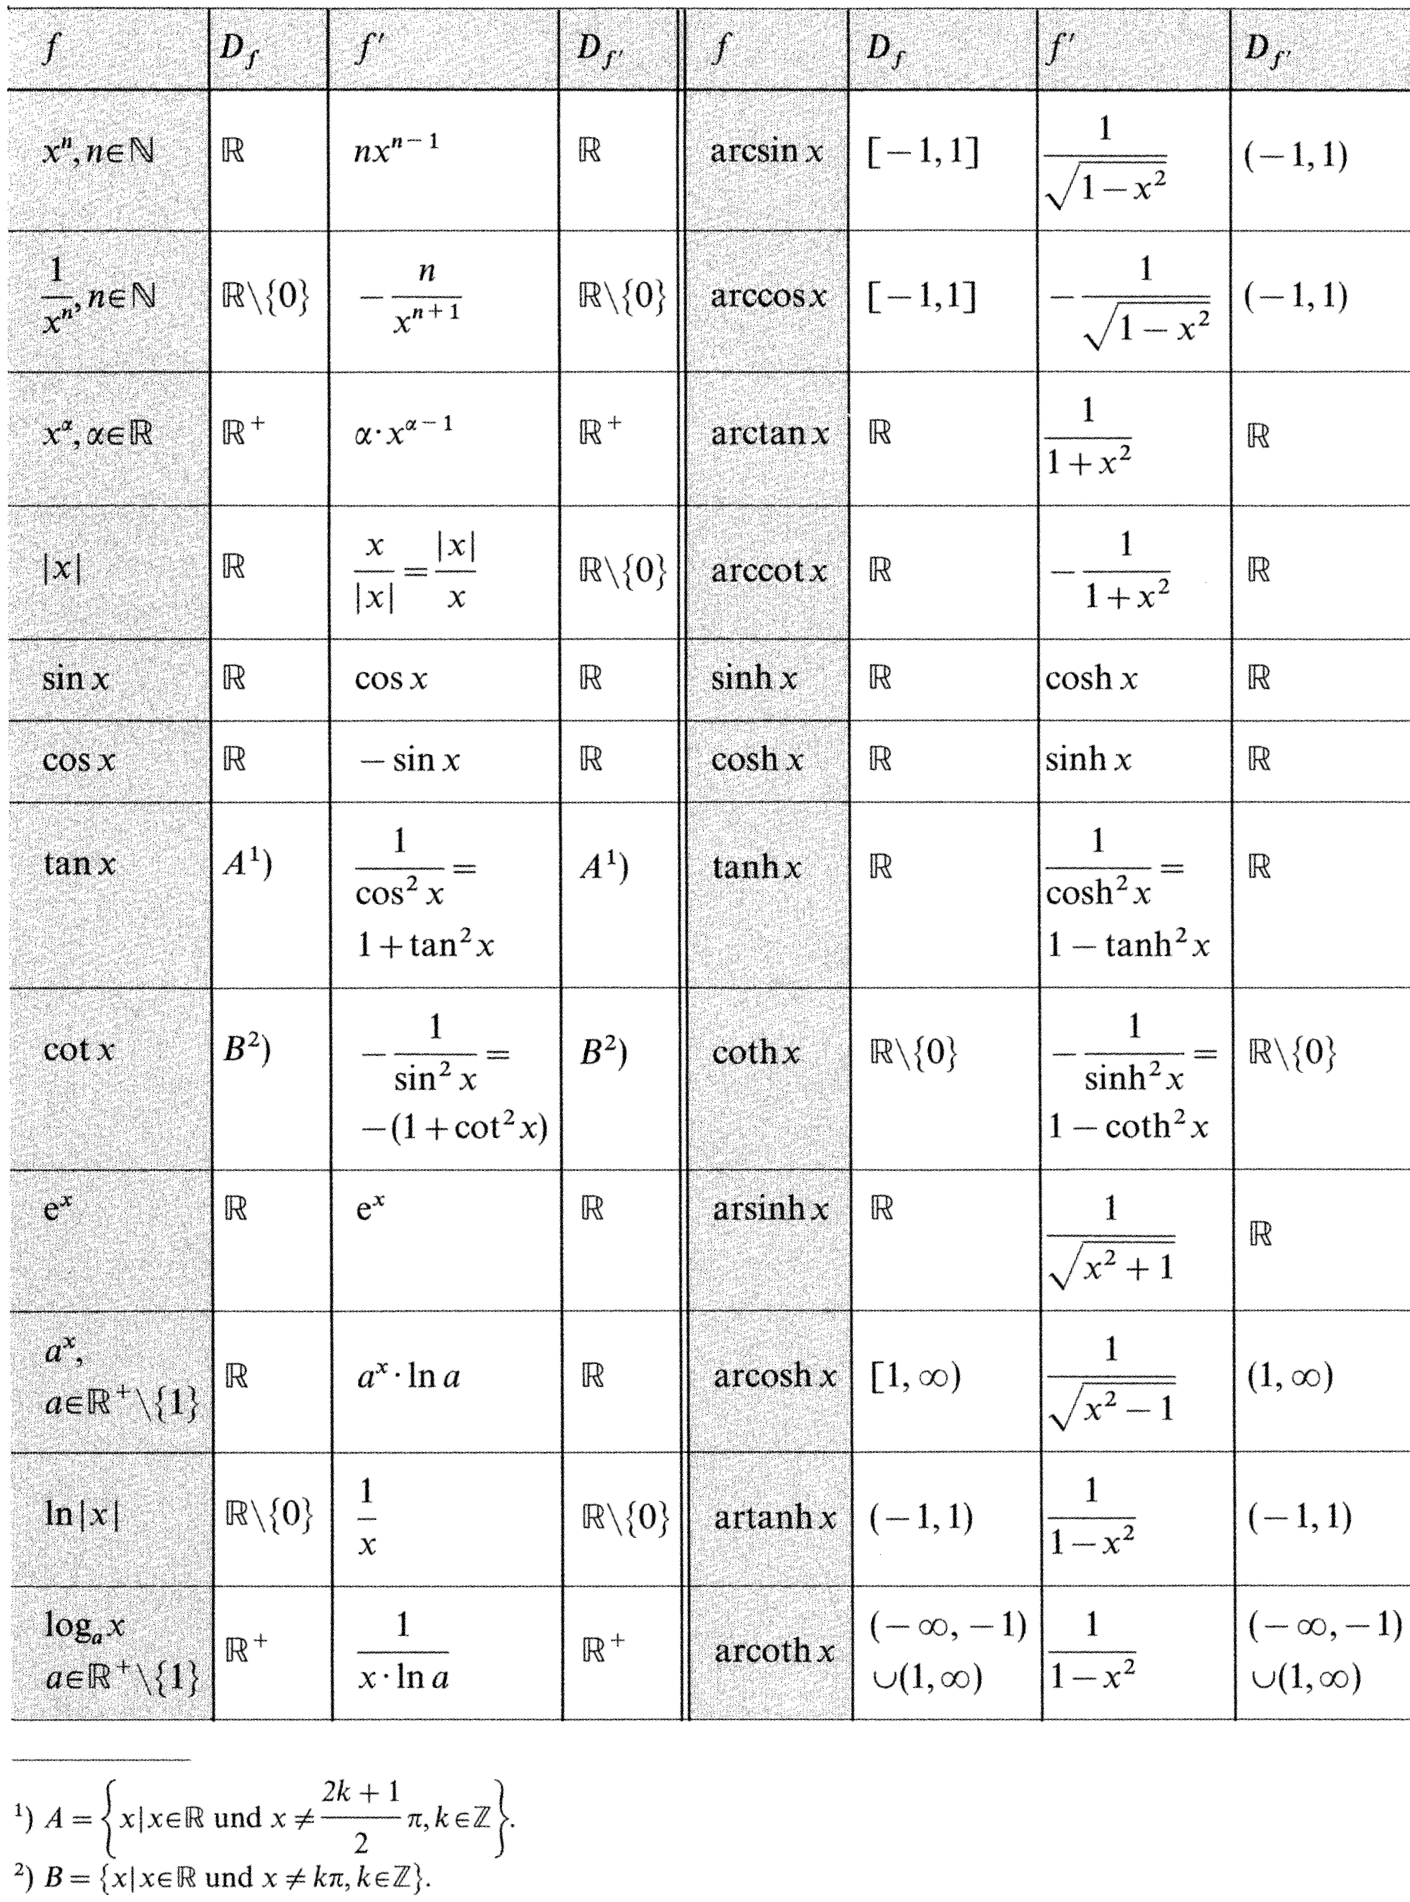
\includegraphics[width=\columnwidth]{images/V0B0.png}